% !TeX encoding = UTF-8
\section{Begriffliche Annäherung}

Der Begriff Trauma entstammt dem Griechischen und bedeutet Wunde oder Verletzung (vgl. Landolt \& Hensel 2008: 14). Dabei wird nicht unterschieden, ob der Körper oder die Seele betroffen ist (vgl. ebd.). Folgendes Kapitel stellt eine erste Annährung an die Beantwortung der Frage dar, was Traumapädagogik sei. Dazu ist der Begriff \textit{Trauma} zu erklären (1.1), was nicht eindeutig möglich ist. Danach werden die in der Literatur vorfindlichen Definitionen der Traumapädagogik vorgestellt (1.2.). Das Kapitel schließt, indem die Entstehung und Institutionalisierung der Traumapädagogik beschrieben werden (1.3).

\subsection{Trauma}
Trauma ist ein Begriff, der in den letzten Jahren sowohl im Alltagsgebrauch als auch in verschiedenen psychosozialen Handlungsfeldern sehr populär geworden ist. Im allgemeinen Sprachgebrauch wird unter Traumatisierung meist eine seelische Verletzung verstanden (vgl. Hantke \& Görges 2012: 53). Der Begriff wird selbst in der Traumaforschung nicht eindeutig benutzt. Nicht immer wird deutlich, ob Trauma das Ereignis, die Auswirkungen, die Symptome oder das Leiden bedeutet (vgl. ebd). Die International Classification of Diseases (Internationale statistische Klassifikation der Krankheiten und verwandter Gesundheitsprobleme, kurz ICD, momentan gültige Fassung: ICD-10) definiert Trauma indirekt als ein „Ereignis oder eine Situation kürzerer oder längerer Dauer, mit außergewöhnlicher Bedrohung oder katastrophenartigem Ausmaß, die bei fast jedem eine tiefe Verzweiflung hervorrufen würde“ (ICD-10-GM 2016, F43.1). Im Diagnostic and Statistical Manual of Mental Disorders (zu Deutsch: Diagnostischer und statistischer Leitfaden psychischer Störungen, Fassung DSM-IV-TR) werden zwei Aspekte genannt, die gleichzeitig erfüllt werden müssen, um von Trauma zu sprechen: (1) das Erleben oder Beobachten eines Ereignisses, das eine ernsthafte Bedrohung der körperlichen oder psychischen Integrität der eigenen oder anderer Personen darstellt; (2) die Reaktionen der betroffenen Person sind von intensiver Furcht, Hilflosigkeit, Grauen und durch aufgelöstes oder agitiertes Verhalten begleitet (vgl. Saß u.a. 2003: 512). Im aktuellsten DSM V entfällt das zweite Kriterium, das sich auf das subjektive Erleben bezieht (vgl. Falkai u.a. 2015: 1111). Mit der Entstehung, der Erfassung, dem Verlauf und der Behandlung der Folgen lebensbedrohlicher und/oder extrem belastender Ereignisse befasst sich Psychotraumatologie (vgl. Landolt \& Hensel 2008: 14), die mit ihrer stressbezogenen Sichtweise (vgl. Hensel 2014: 27) von einem kausalen Zusammenhang zwischen dem Entstehen einer psychischen Störung und belastenden Lebensereignissen ausgeht. Laut Hausmann (2006:16) beschäftigt sich Psychotraumatologie mit traumatischen Ereignissen und ihren Auswirkungen auf das Erleben und Verhalten von Einzelpersonen und sozialen Systemen. Ein psychisches Trauma sei dabei als ein zumeist plötzlich auftretendes Ereignis zu verstehen, das auf den Betroffenen sehr bedrohlich wirke und zugleich als nicht zu bewältigen erscheine (vgl. Hausmann 2006: 31). Ein Trauma löst intensive Gefühle des Ausgeliefertseins, der Hilflosigkeit, des Entsetzens, der Angst, Verzweiflung oder Wut aus oder führt zu einem Zustand der emotionalen Betäubung und Apathie. Ein psychisches Trauma kann langfristige psychische Symptome verursachen. Die traumatisierende Wirkung eines Ereignisses hängt von der Art des Geschehens sowie von dessen Umständen ab, aber auch von der betroffenen Person, ihren Handlungs- und Bewältigungsmöglichkeiten sowie verschiedenen Schutz- und Risikofaktoren (vgl. ebd.). Die Schutzfaktoren, die unter die Resilienz subsumiert werden und die die Auswirkungen der traumatischen Situationen abschwächen würden, verlieren laut Hensel an Bedeutung, je intensiver und häufiger die Belastung ist (vgl. Hensel 2014: 27). Die klassischen Diagnosen der Anpassungsstörung sowie die posttraumatische Belastungsstörung (PTBS) sind nicht die einzigen und häufigsten Folgen einer Traumatisierung (vgl. ebd.), obwohl hauptsächlich diese zur Verfügung stehen. Zu den typischen PTBS-Symptomen gehören, die traumatischen Erlebnisse in Form von Bildern, Gedanken, Wahrnehmungen oder Halluzinationen (sog. \textit{Flashbacks}) wiederholt zu erleben; mit dem Trauma verbundene Reize zu vermeiden; übertriebene Wachsamkeit. Fehlen diese Symptome, ist dies jedoch keine Garantie dafür, dass kein Trauma vorliegen kann (vgl. Becker 2006: 175). Zu traumatischen Erfahrungen zählen nach klassischem Verständnis hauptsächlich lebensbedrohliche Ereignisse, sexueller Missbrauch oder Misshandlung (vgl. Hensel 2014: 27). Zu chronischen psychischen Fehlanpassungen tragen unter anderem auch solche extremen Belastungen wie der Verlust einer wichtigen Bezugsperson (nicht nur durch Tod) sowie immer wieder im Alltag erlebte Kränkungen (wie Ausgrenzung, psychische Misshandlung und Mobbing) bei (vgl. ebd.). Potenziell traumatisierende Ereignisse sind von unterschiedlicher Art und Dauer. Die amerikanische Kinderpsychiaterin Leonore Teer (1991 zit. nach Landolt \& Hensel 2008: 14) unterscheidet zwei Arten von Traumata:

\begin{itemize}[noitemsep]
\item Typ I - einmalige, zeitlich begrenzte, zufällige Traumata (z.B. Naturkatastrophen, Verkehrsunfälle oder Brandkatastrophen), sogenannte Monotraumata
\item Typ II - länger andauernde und wiederholte, teilweise vorhersehbare Geschehnisse (z.B. Sexueller Missbrauch, familiäre Gewalt, Aufenthalt im Kriegsgebiet), sprich: multiple Traumata
\end{itemize}

Des Weiteren können traumatisierende Ereignisse anhand ihrer Ursache klassifiziert und in von Menschen verursachte Ereignisse („man made“) oder durch Naturkatastrophen hervorgerufene und akzidentelle Traumata (z.B. ein Autounfall) eingeteilt werden (vgl. Landolt \& Hensel 2008: 15, siehe Abbildung 1). Dabei geht es immer um ein Ereignis, das eine Bedrohung für das Leben und die körperliche Unversehrtheit des Menschen darstellt (vgl. ebd.). Die neurobiologischen Befunde lassen davon ausgehen, dass traumatische Ereignisse auf der Ebene des Gehirns eine gestörte Informationswahrnehmung bedeuten können (vgl. Landolt \& Hensel 2008: 16).

\begin{figure}[h]
  \centering
  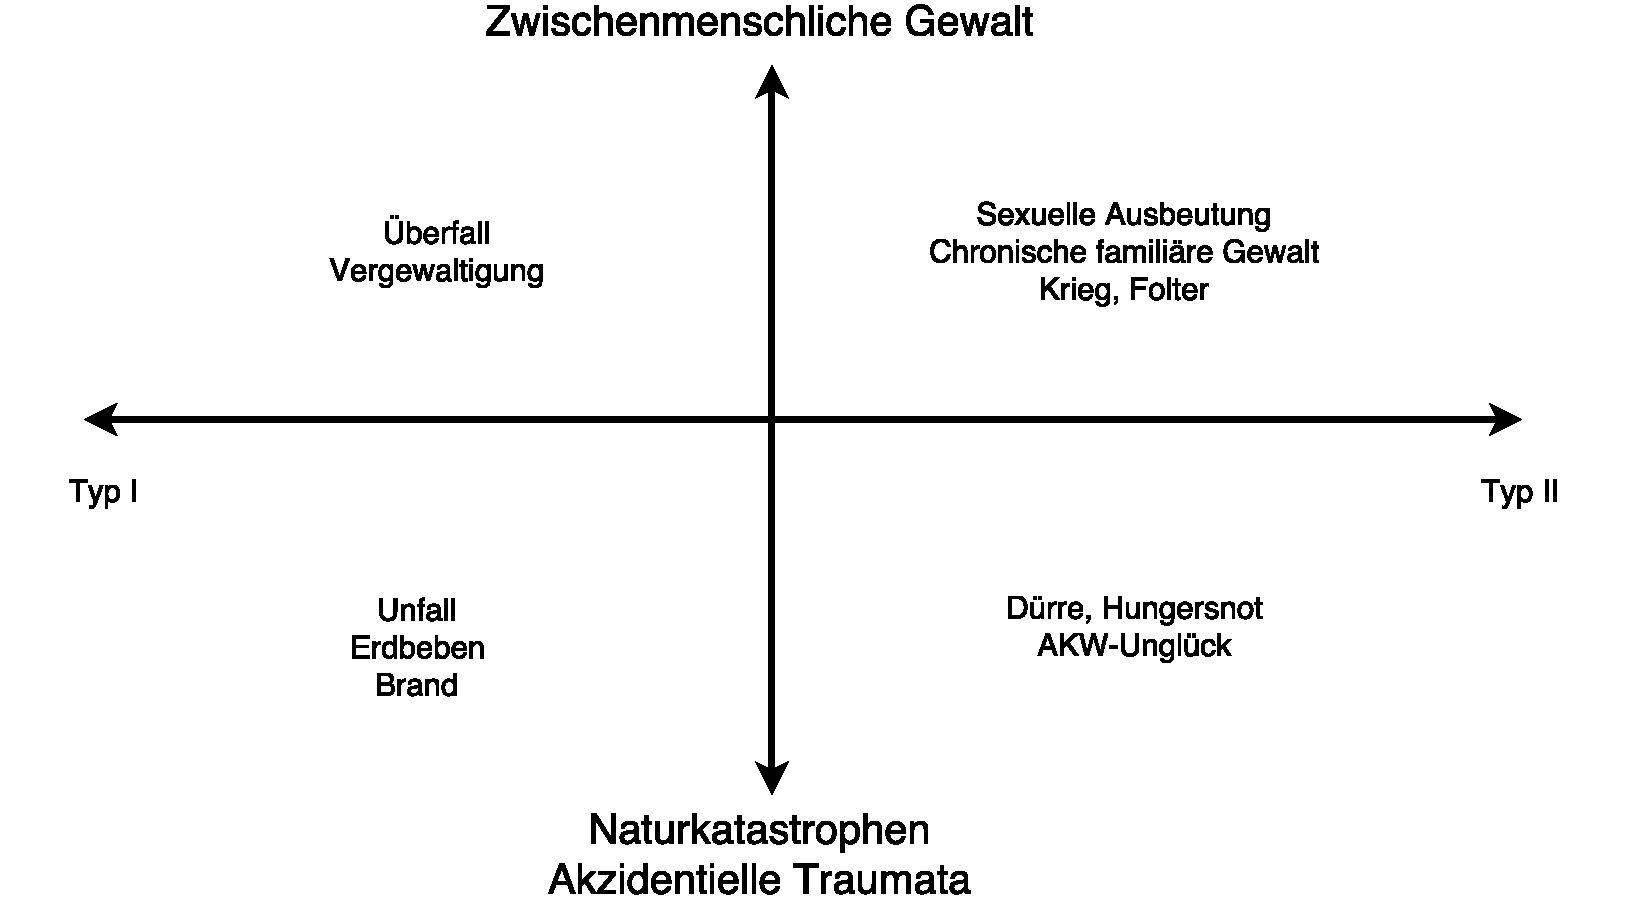
\includegraphics[scale=0.5]{abbildung1}
  \caption
      [Klassifikation traumatischer Ereignisse]
      {Klassifikation traumatischer Ereignisse (nach Landolt, 2004 zit. nach Landolt \& Hensel 2008: 14)}
\end{figure}

Die Entwicklung einer posttraumatischen Reaktion ist als Folge realer Erfahrungen und nicht als Eigenart des Individuums zu verstehen (vgl. Hensel 2014: 28). „Es sind die konkreten Lebensbedingungen, die psychische Symptome verursachen; es sind unbewältigte Lebenserfahrungen im Sinne einer Traumageschichte, die psychisch krank machen. Nur Störungen zu sehen, ohne den Hintergrund der Entstehung zu erkennen und anzuerkennen, bedeutet die Person zu pathologisieren“ (Huber 2003: 31). Diese Sichtweise ist keineswegs neu. Sie knüpft an die Anfänge der Psychotherapie (Psychoanalyse) und der freudschen Erkenntnis des Zusammenhangs zwischen der Erfahrung des sexuellen Missbrauchs in der frühen Kindheit und den Symptomen (Hysterie) im Erwachsenenalter an (vgl. Hensel 2014: 29f.). Nach Freud ist ein Trauma „ein Erlebnis, welches dem Seelenleben innerhalb kurzer Zeit einen so starken Reizzuwachs bringt, dass die Erledigung oder Aufarbeitung derselben in normal-gewohnter Weise missglückt, woraus dauernde Störungen im Energiebetrieb resultieren müssen“ (Freud 1961: 284). 

\subsection{Traumapädagogik - Begriff und Definition}
Traumapädagogik wird als „Sammlungsbegriff für [...] Konzepte [benutzt], um die Handlungsfähigkeit der professionellen Fachkräfte wieder herzustellen und traumatisierten Kindern, Jugendlichen und Erwachsenen eine adäquate Teilhabe am sozialen Leben zu ermöglichen“ (Website Traumapädagogik o.J., vgl. Bausum u.a. 2013: 8). Aus den psychotraumatologischen Erkenntnissen sind, so Bausum, abgeleitete Konzeptionen entstanden, die in ihrer Komplexität als eigenständige „Fachrichtung der Traumapädagogik“ zu verstehen seien (ebd.).  

Der Begriff \textit{Traumapädagogik} bleibt schwammig und wird zum Teil unterschiedlich benutzt (vgl. Schmid u.a. 2007: 333). Der Begriff selbst ist vermutlich auf Volker Vogt und Martin Kühn zurückzuführen, die 2002 ein Webprojekt (www.traumapädagogik.de) als ein Diskussionsforum zur kindlichen Traumatisierung in der Pädagogik initiierten (vgl. Kühn 2006: 4; Weiß 2016b: 22). Kühn (2006: 5) distanzierte sich mit der Zeit von der anfangs als Arbeitstitel gedachten Bezeichnung seines Projektes. Der Name \textit{Traumapädagogik} zeige nicht deutlich genug, wozu und mit welchem Ziel gewirkt werden solle. Im Falle seines Konzeptes entscheidet er sich dafür, von einer \textit{Pädagogik} des sicheren Ortes zu sprechen (vgl. Kühn 2006: 4 f.). Kühn definiert Traumapädagogik als Ansatz zur Stabilisierung und Förderung traumatisierter Kinder und Jugendlicher. Sie sei eine notwendige Voraussetzung, Begleitung und Ergänzung eines entsprechenden Therapieprozesses. Daraus ergibt sich die Notwendigkeit eines engen interdisziplinären Austauschs und Diskurses zwischen Pädagogik, Psychotherapie und Psychiatrie (vgl. Kühn 2013: 27). Schmid versteht Traumapädagogik als „die konsequente Anwendung des aktuellen Kenntnisstands der Psychotraumatologie auf das pädagogische Verständnis der betreuten Menschen“ (Schmid 2013: 46). Damit meint er vor allem traumapädagogische Konzepte in der stationären Jugendhilfe als Beispiel für „die konsequente Umsetzung eines innovativen pädagogischen Konzepts, das auf klare psychopathologische Symptome abzielt“ (Schmid 2013: 57). Gemäß seinem Verständnis ist Traumapädagogik eine symptomspezifische, pädagogische Förderung psychisch belasteter Kinder und Jugendlicher (vgl. Schmid 2013: 57). Schmid u. a. (2007: 333) bemängeln, dass der Begriff häufig rein theoretisch besetzt werde, ohne daraus praktische Handlungskonsequenzen oder pädagogische Konzepte abzuleiten. Die Traumapädagogik entstand hauptsächlich an der Schnittstelle zwischen Kinder- und Jugendpsychiatrie/-psychotherapie und Jugendhilfe, die geholfen hat, „aus der Psychotraumatologie heraus milieutherapeutische Konzepte abzuleiten oder althergebrachte Konzepte der Heimerziehung aus einer psychotraumatologischen und neurobiologischen Perspektive heraus zu begründen“, so Schmid u.a. (2014: 174). Weiß (2016b: 29) sieht die Möglichkeit, die Haltungen und Methoden der Traumapädagogik vielseitig anzuwenden. Eine traumapädagogische Haltung sei eine solche, die für jede Pädagogik gültig sein sollte. Denn extremer Stress und traumatische Erfahrungen seien im Leben vieler Menschen verbreitet (vgl. ebd.). Weiß betont den Unterschied zwischen einerseits der Traumabearbeitung als der Bewältigung durch die Betroffenen und andererseits der Traumaarbeit, die die Begleitung durch psychosoziale Fachkräfte sei (vgl. Weiß 2016b: 20 f.). Sie versteht Traumapädagogik als notwendige Unterstützung traumatisierter Kinder und Jugendlicher im pädagogischen Alltag als Teil der Traumaarbeit (vgl. ebd.). Weiß u. a. definieren Traumapädagogik als eine junge Fachrichtung, die es sich zur Aufgabe gemacht hat, Fachkräfte, die mit traumatisch belasteten Kindern und Jugendlichen im Arbeitsalltag konfrontiert sind, zu unterstützen (vgl. Weiß u.a. 2016: 11). Dies soll durch spezifische Fort- und Weiterbildungen und die Schaffung tragfähiger Strukturen in den Institutionen geschehen (vgl. ebd.). Die Traumapädagogik sei als Antwort auf die Fragen der Praxis nach dem Umgang mit traumatisch belasteten Kindern und Jugendlichen in pädagogischen Arbeitsfeldern entstanden und fokussiere in der Auseinandersetzung mit dieser Frage drei Bereiche (vgl. Bausum u.a. 2013: 8):

\begin{itemize}[noitemsep]
\item Begegnung zwischen Kind und pädagogischer Fachkraft 
\item Handlungssicherheit der pädagogischen Fachkraft 
\item Institutionelle Strukturen der Einrichtung
\end{itemize}

Die vorhandenen Definitionen der Traumapädagogik zeigen, dass diese noch ganz in den Anfängen steckt und anscheinend um ihre Berechtigung und Anwendungsbereiche kämpft. Die Traumapädagogik, trotz direkter Bezüge zur Psychotraumatologie, sagt nicht immer eindeutig aus, was unter Traumatisierung verstanden wird, was es wiederum erschwert, den Gegenstand und die Handlungsfelder zu bestimmen.

\subsection{Entstehung und Institutionalisierung der Traumapädagogik}
Die Anfänge der heute unter dem Begriff Traumapädagogik subsumierten Konzepte sind in stationären und teilstationären Einrichtungen der Kinder- und Jugendhilfe ab Mitte der 1990er-Jahre zu suchen (vgl. Weiß 2016b: 20). Ihnen vorausgegangen sind Ende der 1980er-Jahre Prozesse der Enttabuisierung des Themas sexueller Gewalt in der Kinder- und Jugendhilfe und folglich die Erweiterung des Blickwinkels auf andere Formen der Gewalt gegen Kinder. Stationäre Jugendhilfe, Pflegeeltern und Behindertenhilfe sind Bereiche, die Bedarf an entsprechenden Konzepten außerhalb des psychotherapeutischen Rahmens melden (vgl. Weiß 2016b: 20 f.).

Der Prozess der Professionalisierung und Institutionalisierung der Traumapädagogik beginnt zu Anfang dieses Jahrhunderts mit ersten Publikationen, Fort- und Weiterbildungen bis hin zur Gründung einer Bundesarbeitsgemeinschaft Traumapädagogik (BAG-TP), die sich zum Ziel setzt, das psychotraumatologische Wissen in verschiedene pädagogische Arbeitsfelder in Form von Diskussionen und Fortbildungen in traumabezogener Pädagogik zu tragen. Ihre Ziele sieht die BAG-TP in „Entwicklung, Förderung und Forschung von/zu Konzeptionen und Projekten in Erziehungs-, Bildungseinrichtungen und der Jugend-/Behindertenhilfe. Themen sind dabei u.a. die psychischen, physischen, sozialen und gesellschaftspolitischen Grundlagen und Folgen von Stressreaktionen bei Kindern und Jugendlichen auf traumatische Lebensereignisse und entsprechenden pädagogischen Begegnungen und Interventionsmöglichkeiten“ (BAG-TP 2011: 2). BAG-TP formuliert 2011 Traumapädagogische Standards in der stationären Kinder- und Jugendhilfe sowie, zusammen mit der Deutschsprachigen Gesellschaft für Psychotraumatologie (DeGPT), Kriterien für ein Curriculum Traumapädagogik/Traumazentrierte Fachberatung. Nach einer entsprechenden Weiterbildung, die momentan an 36 Instituten in Deutschland angeboten wird (vgl. DeGPT/Fachverband Traumapädagogik o.J.), kann eine Qualifikation für Traumapädagogik/Traumazentrierte Fachberatung erworben werden.

Hantke (2012: 198) beschreibt den Prozess der Entstehung der Traumapädagogik und ihrer Institutionalisierung vor dem Hintergrund der Ausdifferenzierung und Entgrenzung der therapeutischen, beraterischen und pädagogischen Bereiche. Die neuen Überlegungen, die aus der Traumatheorie resultieren, wurden in erste therapeutische Verfahren umgesetzt und diese dem Bereich der psychologischen Psychotherapie zugeschrieben. Damit sei der Zugang zu dem neuen Wissen und den Verfahren für viele psychosoziale Fachkräfte begrenzt gewesen. Die neuen, traumazentrierten Methoden, Denk- und Erklärungsansätze sollen Einzug in die stationäre Versorgung und in ambulante Settings in Form neu entstehender Traumapädagogik- und Traumaberatungscurricula gefunden haben (vgl. ebd.).
